%* Analysis results - Morten
%	- Capabilities compared to existing systems
%\section{Comparision to other systems}

%	- Is it useful/not useful?
%	- What does our system prove from research standpoint?

%not implemented
\section{Not implemented}
Because this project had a limited timeframe there is a couple of things
we thought could be a good idea to have in the
music streamer, but we did not have the time to implement.

\subsection{Bad Health List}
A robust and distributed system needs some way to keep content on the network in good health,
meaning that there are sufficiently many peers hosting it.
We wanted to maintain a list on the DHT containing the various songs which need additonal peers seeding it,
and make each peer seed at least 5 of such bad health items.
This bad health list system was implemented, but was we did not have enough time to properly test it,
it was been left as a comment in the app.component file.


\subsection{Resource Management}
When the storage capacity of a peer is full and the user want to get more songs,
we need a strategy for what content we can throw away to create room for more.
An obvious choice is to iterate through the content we have from the bad health list,
scrape it to see if any of those songs are in good health,
and then remove them.
If there are already many active seeds on one of those songs,
we can throw the content away if we are not using it.
Another choice is to run through all the songs we have downloaded,
and see if some of them are in good health but are seldomly played so they could be deleted.

We might also implement active resource management, which checks how often songs are used,
and find those songs that are rarely used but in good health, and either remove them,
or replace them with a stub containing a magnetURI, 
that the program could automatically redownload on demand.
An active resource management creates additional overhead both on the local machine,
but also on the network, as it would need to break existing peer connections.
Replacing existing content with stubs would be extra costly,
as it would be necessary to create new WebRTC connections,
when the user wishes to listen to a song that was previously downloaded and stored,
but had since been removed by resource management.

%* What did we not implement? - Morten
%	- Seeder eviction
%	- Eviction strategies
%	- Resource limitations
%	- Bad Health supported properly?
%	- Missing features on \acs{GUI} (why there are unused \acs{GUI} source code)
%	- Fake \acs{DHT} impl, what problems it causes
\subsection{Fake \acs{DHT}}
We did not implement a DHT, because we could not find a mature system already implemented we could use, and we did not have time to implement one ourselves.
Our focus was elsewhere.
With a fake \acs{DHT} all the information about what peers have a torrent is on the server. This is a central point of failure, so if our server is taken down our system is not working anymore.
With a distributed \acs{DHT}, we would not be vulnerable to losing our server because the code could just be cached in a browser and run from anywhere.
%	- Missing trackerless feature
\subsection{trackerless torrenting}
It is not possible to make trackerless torrenting using Web-RTC see \ref{sec:trackerless}. Even though it would have been a nice feature to request a torrent only using the \acs{DHT}, it would mean that we would need to use another technology than Web-RTC. 

%	- Could \acs{DHT} and trackerless be implemented with more work?
\section{Tests}
\begin{figure}[H]
	\centering
	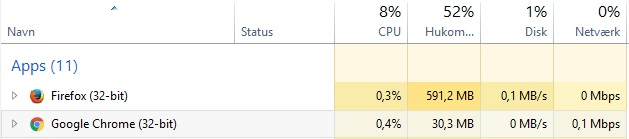
\includegraphics[scale=0.8]{gfx/streamerIdle}
	\caption{The resources spend while running the music streamer}
	\label{fig:streamer-idle}
\end{figure}
The figure \ref{fig:streamer-idle} shows how many resources are spend when running the musicstreamer in Google Chrome.

The Spotify desktop application uses 52-53 mb memory compared to running our music-streamer, but having songs in the localstorage of the browser increses the memory used. In Mozilla Firefox having two songs stored in the local storage and running the music streamer uses 370mb memory.

The difference is that we need to use the local storage of the browser to save the songs.
Spotify have their servers where the music is stored, but we need each peer to store its own music.
%\begin{table}[]
%\centering
%\caption{The amount of memory spend by the music-streamer while adding more songs}
%\label{tab_memUsage}
%\begin{tabular}{lllll}
%0 & 14,9  \\
%1 & 35 \\
%2 & 57,9 \\
%3 & 81,3 \\
%4 & 104 \\
%5 & 126\\
%6 & 149\\
%7 & 172\\
%8 & 195\\
%9 & 218\\
%10 & 240\\
%11 & 263\\
%\end{tabular}
%\end{table}

We have used heap snapshots in Google Chrome to get a picture of how much memory the streamer is using when idle and when we add songs to it. In \ref{fig:memoryUsage} we have made an experiment where we add the same song to the streamer ten times to see if the memory increase is deterministic.
\begin{figure}[H]
	\centering
	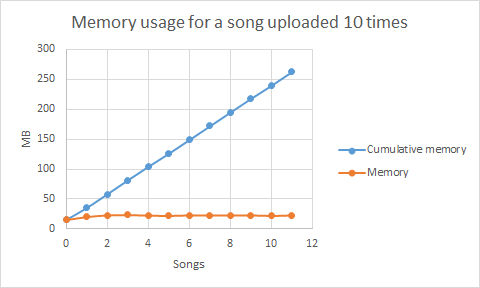
\includegraphics[scale=0.9]{gfx/memoryUsage}
    \caption{A graph over the memory usage when adding the {\em same} song 10 times to the streamer}
	\label{fig:memoryUsage}
\end{figure}
\noindent
As can be seen on the figure that is the case, and the memory is increasing lineary.
\begin{figure}[H]
	\centering
	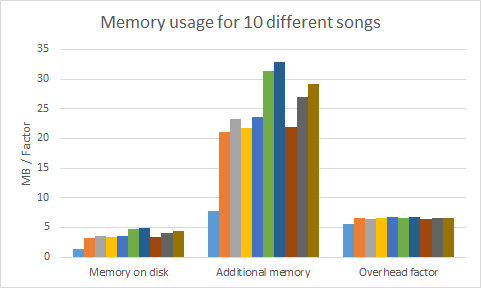
\includegraphics[scale=0.9]{gfx/memoryDiffSize}
	\caption{The memory spend when adding 10 different sized songs}
	\label{fig:memoryDiffSizes}
\end{figure}
\noindent
Figure~\ref{fig:memoryDiffSizes} show an experiment where we upload a song to the streamer and reset the storage before we upload another different song. The experiment shows how much space takes on the disk and how much it takes in the music-streamer. As we can see each song takes about six times more space in the music-streamer, but an important thing to notice is that the songs are stored derterministic so storing 1 MB of data alway takes around $\sim6.5$ MB of data on the server for all the songs.

We have run the experiments a couple of times to make sure the result was not just random, but was following a general trend. In the graphs we used the av
%TODO
%* Quantifiable Tests (Reproducible) (performance, robustness) - Morten
%	- CPU utilization when using/not using parts of project?
%	- LocalStorage performance degredation?
%	- Memory use?
%	- Comparison with spotify/others
%	- Reported traffic by webtorrent
%		Is it correct+complete?
